\section{Cook}\label{sec:cook} % (fold)

Für die Reproduktion des Workflows mit identischer Einrichtung werden zwei Programme benötigt: nginx
als Reverse Proxy sowie Docker zur Ausführung des n8n-Containers und der MongoDB-Datenbank.


Im bereitgestellten ZIP-Archiv befindet sich die Datei \verb|nginx.conf|. In dieser Datei ist in Zeile 4
und in Zeile 13 der korrekte Domainname einzutragen. In Zeile 10 und in Zeile 11 sind der Pfad zum
SSL-Zertifikat und der Pfad zum zugehörigen privaten Schlüssel anzupassen. Nach der Anpassung wird
die Datei in das Verzeichnis \verb|/etc/nginx/sites-available| kopiert und mit einem aussagekräftigen
Namen, beispielsweise n8n, versehen. Anschließend wird im Verzeichnis
\verb|/etc/nginx/sites-enabled| ein
symbolischer Link auf die Konfigurationsdatei erstellt:

\begin{verbatim}
ln -s /etc/nginx/sites-available/n8n /etc/nginx/sites-enabled/n8n
\end{verbatim}

Damit die Änderungen wirksam werden, ist der nginx-Dienst neu zu laden:

\begin{verbatim}
nginx -s reload
\end{verbatim}

Im entpackten ZIP-Archiv befindet sich ebenfalls die Datei \verb|.env.example|. Diese ist in
\verb|.env| umzubenennen. In der Datei wird der Domainname eingetragen. Der Start von n8n und
MongoDB erfolgt über den folgenden Befehl:

\begin{verbatim}
docker compose up
\end{verbatim}

Standardmäßig wird dabei die aktuelle stabile Version von n8n verwendet. Die gewünschte Version kann
in der Datei \verb|docker-compose.yml| festgelegt werden. Die zuletzt getestete Version ist
\verb|1.105.3|.

Beim ersten Aufruf des n8n-Servers wird die Erstellung eines Benutzerkontos abgefragt. Nach
erfolgreichem Abschluss der Registrierung erfolgt die Weiterleitung zur Übersichtsseite, die
\autoref{fig:n8n_overview} dargestellt ist.

\begin{figure}
    \begin{center}
        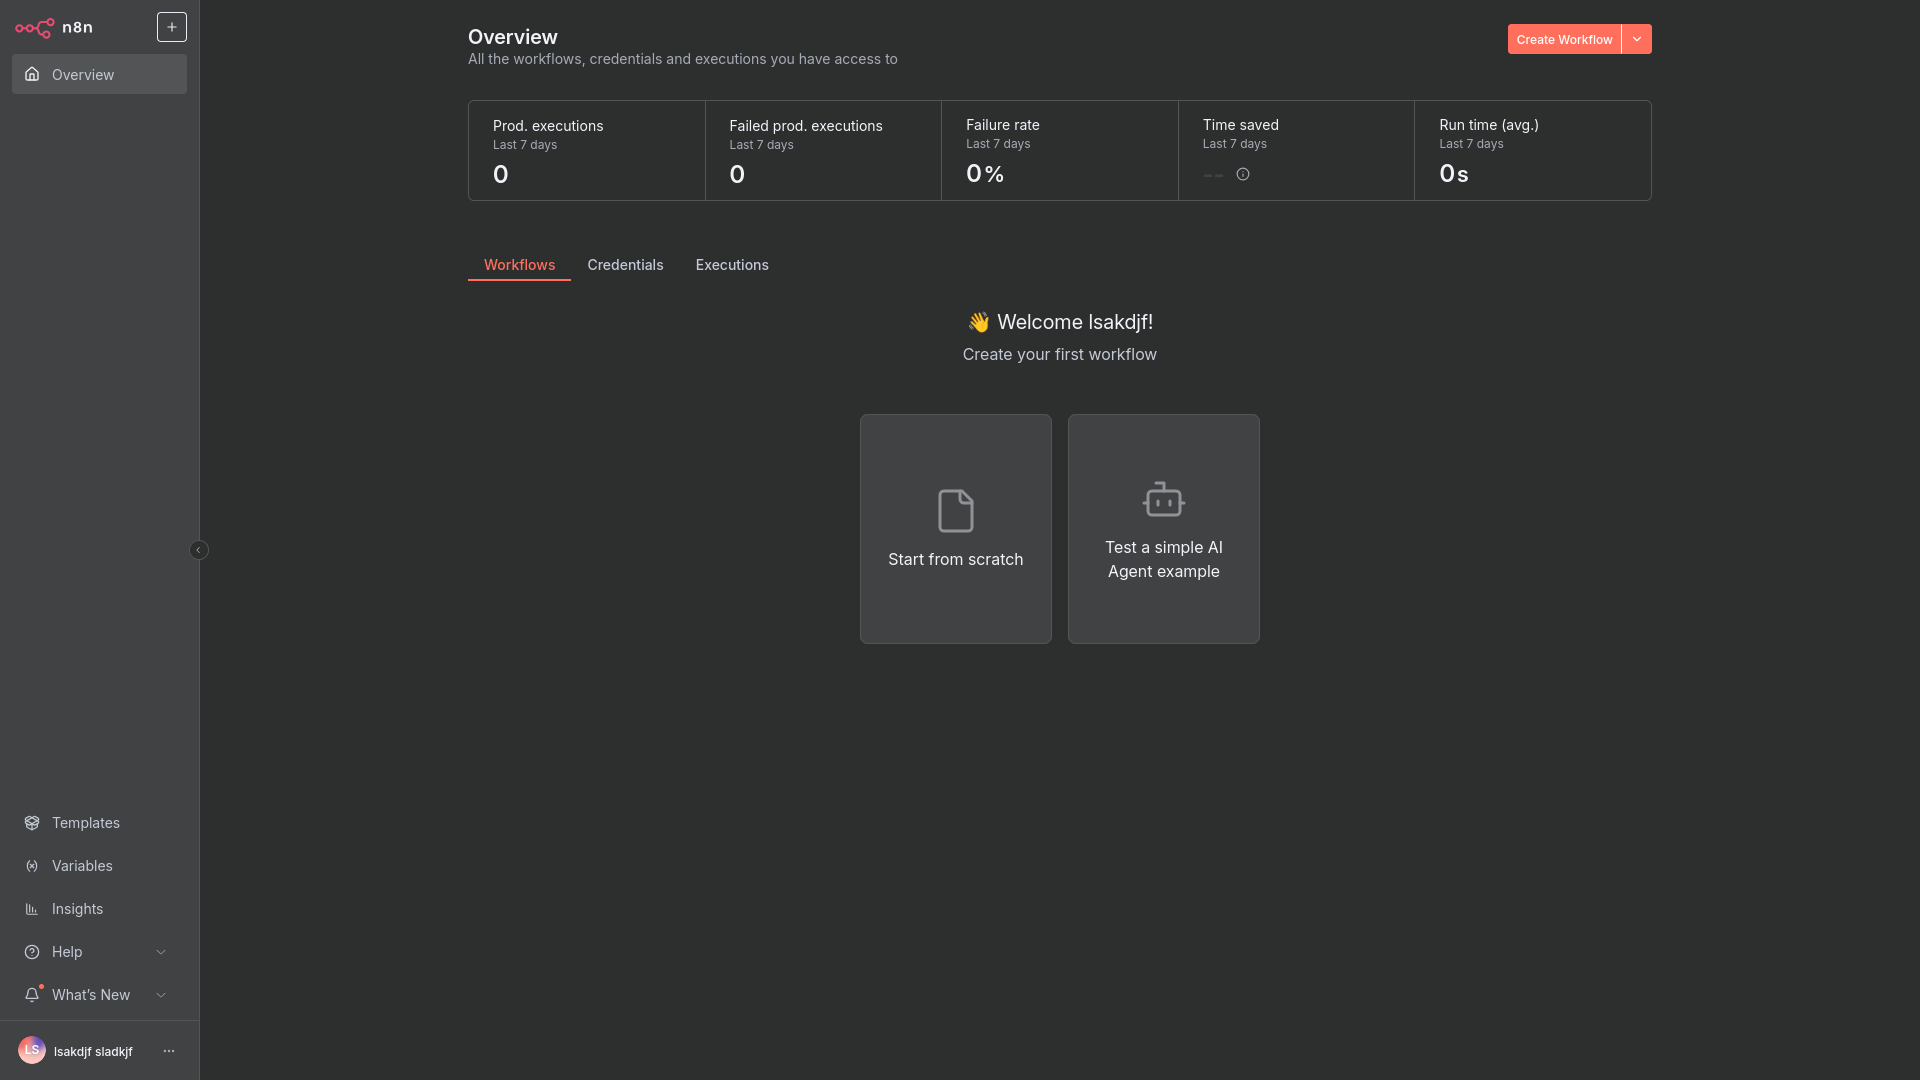
\includegraphics[width=0.95\textwidth]{images/n8n_overview.png}
    \end{center}
    \caption{n8n Übersichtsseite}\label{fig:n8n_overview}
\end{figure}

% section Cook (end)
